\documentclass[11pt, a4paper, oneside]{Thesis} % Paper size, default font size and one-sided paper
\usepackage{wrapfig}
\usepackage{lscape}
\usepackage{rotating}
\usepackage{graphicx}
\usepackage{caption}
\usepackage{amsmath}
\usepackage{listings}
\usepackage{xcolor}
\usepackage{pdfpages}

\definecolor{codegreen}{rgb}{0,0.6,0}
\definecolor{codegray}{rgb}{0.5,0.5,0.5}
\definecolor{codepurple}{rgb}{0.58,0,0.82}
\definecolor{backcolour}{rgb}{0.95,0.95,0.92}

\lstdefinestyle{mystyle}{
    backgroundcolor=\color{backcolour},   
    commentstyle=\color{codegreen},
    keywordstyle=\color{magenta},
    numberstyle=\tiny\color{codegray},
    stringstyle=\color{codepurple},
    basicstyle=\ttfamily\footnotesize,
    breakatwhitespace=false,         
    breaklines=true,                 
    captionpos=b,                    
    keepspaces=true,                 
    numbers=left,                    
    numbersep=5pt,                  
    showspaces=false,                
    showstringspaces=false,
    showtabs=false,                  
    tabsize=2
}

\lstset{style=mystyle}

% prints author names as small caps
\usepackage{hyperref}

% optimization eqn package
% \usepackage{optidef}
\DeclareCaptionJustification{justified}{\leftskip=0pt \rightskip=0pt \parfillskip=0pt plus 1fil}
\captionsetup{font=normalsize,justification=justified}

%\usepackage{subcaption} %incompatible with subfig
\graphicspath{{Pictures/}} % Specifies the directory where pictures are stored
\lstset{inputpath={Codes/}} % Specifies the directory where codes are stored 
\usepackage[utf8]{inputenc}
\usepackage[english]{babel}
\usepackage[square, numbers]{natbib} % Use the natbib reference package - read up on this to edit the reference style; if you want text (e.g. Smith et al., 2012) for the in-text references (instead of numbers), remove 'numbers' v
\usepackage{fancyhdr}
\hypersetup{urlcolor=black, colorlinks=true} % Colors hyperlinks in blue - change to black if annoyingv`	
\title{\ttitle} % Defines the thesis title - don't touch this

\begin{document}
\makeatletter
\renewcommand*{\NAT@nmfmt}[1]{\textsc{#1}}
\makeatother


\frontmatter % Use roman page numbering style (i, ii, iii, iv...) for the pre-content pages

%\setstretch{1.6} % Line spacing of 1.6 (double line spacing)

% Define the page headers using the FancyHdr package and set up for one-sided printing
\fancyhead{} % Clears all page headers and footers
\rhead{\thepage} % Sets the right side header to show the page number
\lhead{} % Clears the left side page header

\pagestyle{fancy} % Finally, use the "fancy" page style to implement the FancyHdr headers
\fancyhf{}
\rhead{\thepage}
\newcommand{\HRule}{\rule{\linewidth}{0.5mm}} % New command to make the lines in the title page

% PDF meta-data
\hypersetup{pdftitle={\ttitle}}
\hypersetup{pdfsubject=\subjectname}
\hypersetup{pdfauthor=\authornames}
\hypersetup{pdfkeywords=\keywordnames}

% Edit fields using Thesis.cls (Don't alter anything else in cls script)

%----------------------------------------------------------------------------------------
%	TITLE PAGE
%----------------------------------------------------------------------------------------

\begin{titlepage}
\begin{center}

\HRule \\[0.4cm] % Horizontal line
{\huge \bfseries \ttitle}\\[0.4cm] % Thesis title
\HRule \\[1.5cm] % Horizontal line
\large \textit{A Thesis Submitted\\ In Partial Fulfillment of the Requirement\\ for the Degree Of\\ \degreename}\\[0.3cm] % University requirement text
\textit{by}\\[0.4cm]

\href{http://home.iitk.ac.in/~username}{\authornames}

(\rollno)\\ to the

\vfill
\graphicspath{ {./Pictures/} }
\begin{figure}[hb]
  \centering
  
\includegraphics[width=0.4\linewidth]{redlogo.jpg}
\end{figure}

\textbf{\DEPTNAME}\\ % Research group name and department name
\textsc{ \UNIVNAME}\\[1.5cm] % University name
\large {\submit}\\[2cm] % Date


\end{center}
\end{titlepage}

% comment below to add certificate through pdf file and not Latex
%--------------------------------------------------------------------------------------
\Certi{{\vspace{1em}} % Add a gap in the Contents, for aesthetics
\setcounter{page}{2}
It is certified that the work contained in this thesis entitled ``\ttitle'' by ``\authornames'' has been carried out under our supervision and that it has not been submitted elsewhere for a degree.
\\[2cm]

\begin{minipage}{0.4\textwidth}
	\begin{flushleft} \large
		%\emph{\large {July, 2020}}\\[2cm] % Date
	\end{flushleft}
\end{minipage}
\begin{minipage}{0.6\textwidth}
	{\begin{flushright} \large
		\supname
		\begin{flushright}
			{
			\normalsize{\deptname\\
			\univname}}
		\end{flushright}
	\end{flushright}}
\end{minipage}

% comment if only one supervisor
\vspace{30mm}
\begin{minipage}{0.4\textwidth}
	\begin{flushleft} \large
		{\large {\submit}}\\[2cm] % Date
	\end{flushleft}
\end{minipage}
\begin{minipage}{0.6\textwidth}
	{\begin{flushright} \large
		\cosupname
		% change department here, if co-supervisor is not from your department
		\begin{flushright}
			{
			\normalsize{\deptname\\
			\univname}}
		\end{flushright}
	\end{flushright}}
\end{minipage}
\vfill{}}
\clearpage % Start a new page
%-----------------------------------------------------------------------
% Include pdf pages of scanned certificate and declaration forms
%\includepdf[pages={1}, offset = 85.5 -71.5, scale=0.8]{stampedcerti.pdf}
%\includepdf[pages={1},frame, offset = 71.5 -71.5]{declaration.pdf}

% comment to include scanned Declaration Page and not Latex
%----------------------------------------------------------------------------------------
%	DECLARATION PAGE
%	Your institution may give you a different text to place here
\Declaration{{\vspace{1em}} % Add a gap in the Contents, for aesthetics

This is to certify that the thesis titled ``\ttitle'' has been authored by me. It presents the research conducted by me under the supervision of \supname\ and \cosupname.

To the best of my knowledge, it is an original work, both in terms of research content and narrative, and has not been submitted elsewhere, in part or in full, for a degree. Further, due credit has been attributed to the relevant state-of-the-art and collaborations (if any) with appropriate citations and acknowledgements, in line with established norms and practices.
\\[4cm]

\begin{minipage}{0.4\textwidth}
	\begin{flushleft} \large
%		\emph{\large {July, 2020}}\\[2cm] % Date
	\end{flushleft}
\end{minipage}
\begin{minipage}{0.6\textwidth}
	{\begin{flushright} \large
		\authornames
		\begin{flushright}
			{Programme: BT-MT (DUAL DEGREE)\\ 
			\normalsize{\deptname\\
			\univname\\
			Kanpur 208016}}
		\end{flushright}
	\end{flushright}}
\end{minipage}

\vfill{}}
\clearpage % Start a new page
%----------------------------------------------------------------------------------------
%----------------------------------------------------------------------------------------
%	ABSTRACT PAGE
%----------------------------------------------------------------------------------------

%\addtotoc{Abstract} % Add the "Abstract" page entry to the Contents

\abstract{{\vspace{1em}} % Add a gap in the Contents, for aesthetics
\setcounter{page}{4}
The thesis work includes ....
}

\clearpage % Start a new page

%----------------------------------------------------------------------------------------
%	ACKNOWLEDGEMENTS
%----------------------------------------------------------------------------------------

\setstretch{1.3} % Reset the line-spacing to 1.3 for body text (if it has changed)

\acknowledgements{\addtocontents{toc}{\vspace{1em}} % Add a gap in the Contents, for aesthetics

First and foremost, I would like to extend my sincerest gratitude to my thesis supervisors .............

}
\clearpage % Start a new page

%----------------------------------------------------------------------------------------
%	LIST OF CONTENTS/FIGURES/TABLES PAGES
%----------------------------------------------------------------------------------------

% Important for always right head page number in Chapters and TOC
\fancypagestyle{plain}{%
\fancyhf{} % clear all header and footer fields
\fancyhead[RO,RE]{\thepage} %RO=right odd, RE=right even
\renewcommand{\headrulewidth}{0pt}
\renewcommand{\footrulewidth}{0pt}}
\lhead{\emph{Contents}} % Set the left side page header to "Contents"
\tableofcontents % Write out the Table of Contents
\lhead{\emph{List of Figures}} % Set the left side page header to "List of Figures"
\listoffigures % Write out the List of Figures
\lhead{\emph{List of Tables}} % Set the left side page header to "List of Tables"
\listoftables % Write out the List of Tables

%----------------------------------------------------------------------------------------
%	ABBREVIATIONS
%----------------------------------------------------------------------------------------

\clearpage % Start a new page

\setstretch{1.5} % Set the line spacing to 1.5, this makes the following tables easier to read
\lhead{\emph{Abbreviations}} % Set the left side page header to "Abbreviations"
\listofsymbols{ll} % Include a list of Abbreviations (a table of two columns)
{
\textbf{DOF} & \textbf{D}egrees \textbf{o}f \textbf{F}reedom \\
\textbf{CoM} & \textbf{C}enter \textbf{o}f \textbf{M}ass\\
%\textbf{Acronym} & \textbf{W}hat (it) \textbf{S}tands \textbf{F}or \\
}

%----------------------------------------------------------------------------------------
%	PHYSICAL CONSTANTS/OTHER DEFINITIONS
%----------------------------------------------------------------------------------------
%
%\clearpage % Start a new page
%
%\lhead{\emph{Physical Constants}} % Set the left side page header to "Physical Constants"
%
%\listofconstants{lrcl} % Include a list of Physical Constants (a four column table)
%{
%Speed of Light & $c$ & $=$ & $2.997\ 924\ 58\times10^{8}\ \mbox{ms}^{-\mbox{s}}$ (exact)\\
%% Constant Name & Symbol & = & Constant Value (with units) \\
%}

%----------------------------------------------------------------------------------------
%	SYMBOLS
%----------------------------------------------------------------------------------------

\clearpage % Start a new page
\lhead{\emph{Symbols}} % Set the left side page header to "Symbols"

\listofnomenclature{lll} % Include a list of Symbols (a two column table)
{
$R_{AB}$ & Rotation matrix from frame $A$ to frame $B$ \\
% Symbol & Name & Unit \\

}

%----------------------------------------------------------------------------------------
%	DEDICATION
%----------------------------------------------------------------------------------------
%
\clearpage
\setstretch{1.3} % Return the line spacing back to 1.3
%
 % Page style needs to be empty for this page
\fancyhf{}
\rhead{\thepage}
\dedicatory{Dedicated to someone special} % Dedication text
%
\addtocontents{toc}{\vspace{2em}} % Add a gap in the Contents, for aesthetics

%----------------------------------------------------------------------------------------
%	THESIS CONTENT - CHAPTERS
%----------------------------------------------------------------------------------------

\mainmatter % Begin numeric (1,2,3...) page numbering

\pagestyle{fancy} % Return the page headers back to the "fancy" style

% Include the chapters of the thesis as separate files from the Chapters folder
% Uncomment the lines as you write the chapters

% Chapter Template

\chapter{Introduction} % Main chapter title

\label{Chapter1} % Change X to a consecutive number; for referencing this chapter elsewhere, use \ref{ChapterX}

\lhead{Chapter 1. \emph{Introduction}} % Change X to a consecutive number; this is for the header on each page - perhaps a shortened title

%----------------------------------------------------------------------------------------
%	SECTION 1
%----------------------------------------------------------------------------------------
Robots have moved from being predominantly in factories to our daily lives. The flying drones doing surveillance, cleaning and serving robots, autonomous cars, and underwater vehicles are all common nowadays.

\section{Motivation and Objectives}

The legged robots have shown great potential in locomotion

\begin{figure}[!htb]
\centering
\begin{minipage}{.5\textwidth}
  \centering
  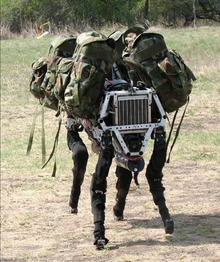
\includegraphics[width=0.65\linewidth]{bigdog.jpg}
  \caption*{(a) BigDog}
\end{minipage}%
\begin{minipage}{.5\textwidth}
  \centering
  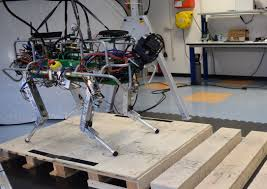
\includegraphics[width=1\linewidth]{hyq.jpeg}
  \caption*{(b) HyQ: Hydraulic Quadruped}
\end{minipage}
\caption[(a) Boston Dynamics' BigDog, (b) HyQ developed by IIT, Genoa, Italy]{(a) Boston Dynamics' BigDog which could carry upto 340 pounds at 4 miles per hour over a rough terrain, which was designed to support military operations, but had issues with noise which was audible from 4 miles away \citep{raibert2008bigdog}, (b) HyQ developed by IIT, Genoa, Italy\citep{semini2011design}}
\end{figure}


\section{Literature Review}

your content here .....\citep{greenwood1997classical}

Some assumption or definition explained in footnote\footnote{My footnote content here}.

\section{Outline}
The thesis focuses on the ....

Chapter \ref{Chapter2} introduces .... Chapter \ref{Chapter3} describes ...

Chapter \ref{Chapter4} focuses on the trajectory optimization .... Later in Chapter \ref{Chapter5}, the results obtained from .... Chapter \ref{Chapter6} provides the conclusion of the work along with the future scope.


% Chapter Template

\chapter{Mathematical Modelling} % Main chapter title

\label{Chapter2} % Change X to a consecutive number; for referencing this chapter elsewhere, use \ref{ChapterX}

\lhead{Chapter 2. \emph{Mathematical Modelling}} % Change X to a consecutive number; this is for the header on each page - perhaps a shortened title

%----------------------------------------------------------------------------------------
%	SECTION 1
%----------------------------------------------------------------------------------------
introduction to the problem... discussing a trivial problem    
\section{Mathematical Preliminaries}

%-----------------------------------
%	SUBSECTION 1
%-----------------------------------
The modelling of a system requires understanding the ... \citep{craig2009introduction}.  

content here ...
\newpage % avoid it in between chapters 

\subsection{Rotation Matrices}
The configuration of a point is completely described by its position vector in $\mathbb{R}^3$, whereas for a rigid body, the orientation of the body in space also needs to be defined.
The orientation of a body-fixed frame $B$ with respect to a reference frame $A$ as shown in Fig. \ref{fig:trans} is given by $R_{AB}$. The rotation matrix that transforms the coordinate frame \textit{A} to coordinate frame \textit{B} has the property:

\begin{equation}\label{eq:ortho}
R_{AB}^{\intercal}\cdot R_{AB} = \mathbb{I}_{3\times 3}.
\end{equation}

\begin{figure}[!htb]
    \centering
    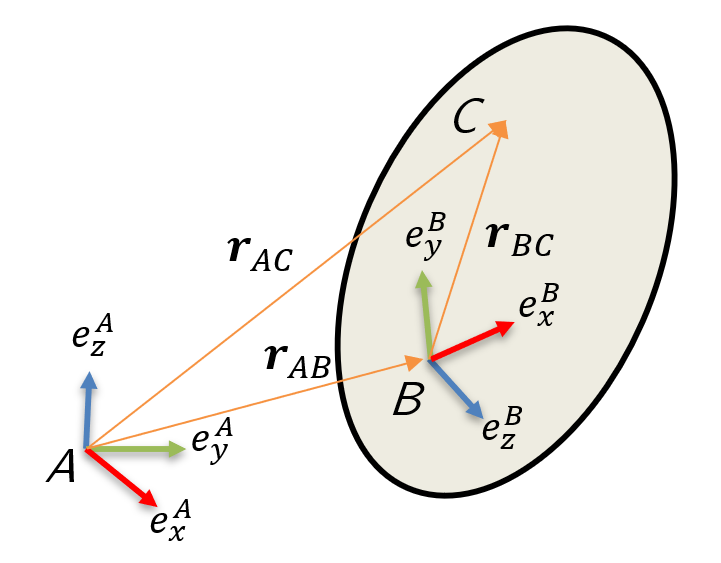
\includegraphics[scale=0.45]{trans_T.PNG}
    \caption{ Coordinate transformations for a single rigid body}
    \label{fig:trans}
\end{figure}

Further, the rotation matrix belongs to a special orthonormal group $SO(3)$, and has properties $R_{AB}^{-1} = R_{BA} = R_{AB}^{\intercal}$.

The orientation of a body could be parametrized in many ways. There are a total of nine parameters in a $3 \times 3$ rotation matrix, but they are constrained by the orthogonality condition of Eq. \ref{eq:ortho}. There are only three independent parameters, and Euler angles are used for a minimal representation of rotations in space.

%----------------------------------------------------------------------------------------
%	SECTION 2
%----------------------------------------------------------------------------------------
 
% Chapter Template

\chapter{Model Design} % Main chapter title

\label{Chapter3} % Change X to a consecutive number; for referencing this chapter elsewhere, use \ref{ChapterX}

\lhead{Chapter 3. \emph{Model Design}} % Change X to a consecutive number; this is for the header on each page - perhaps a shortened title

\section{Robot Model}
.....

\section{Forward Dynamics}

The forward dynamics of the quadruped can be derived using Lagrangian or Newton-Euler method \cite{greenwood1997classical}. 

\subsection{Equation of Motion}\label{EoMderive}
The equation of motion for a rigid multi-body system is usually written in a canonical form \cite{featherstone2014rigid}:
\begin{equation}\label{eq:EoM}
M(\mathbf{q})\mathbf{\dot{u}} + {C}(\mathbf{q,u}) =  \boldsymbol{\tau},
\end{equation}

Refer to Eq. \ref{eq:EoM}

See Appendix \ref{AppendixA}
% Chapter Template

\chapter{Optimization} % Main chapter title

\label{Chapter4} % Change X to a consecutive number; for referencing this chapter elsewhere, use \ref{ChapterX}

\lhead{Chapter 4. \emph{Optimization}} % Change X to a consecutive number; this is for the header on each page - perhaps a shortened title

%----------------------------------------------------------------------------------------
%	SECTION 1
%----------------------------------------------------------------------------------------
your content here .....

Example
See Section \ref{EoMderive} 
% Chapter Template

\chapter{Results and Discussion} % Main chapter title

\label{Chapter5} % Change X to a consecutive number; for referencing this chapter elsewhere, use \ref{ChapterX}

\lhead{Chapter 5. \emph{Results and Discussion}} % Change X to a consecutive number; this is for the header on each page - perhaps a shortened title

%----------------------------------------------------------------------------------------
%	SECTION 1
%----------------------------------------------------------------------------------------

The chapter presents the results of ......
  
\section{Planning and Optimization}\label{PlanResults}

The Y method is used ..... \citep{opencv_library}

Table \ref{tab:params} shows the parameters used in the simulation.
\begin{table}[!htb]
\caption{Parameters used in simulation}
\label{tab:params}
% write to get table number
\begin{center}
\begin{tabular}{ |p{5cm}|p{2cm}|p{3cm}|  }
 \hline
 Robot parameters  &  Symbol & Value\\
 \hline
 Mass & $M$ & 10 Kg\\
 Length & $l$ & 600 mm\\
 Width & $w$ & 420 mm\\
 \hline
\end{tabular}
\end{center}
\end{table}
  
% For MATLAB results, use eps format to add high quality results 

%\begin{figure}[!htb]
%    \centering
%    \includegraphics[trim=90 0 0 0, clip,scale=0.35]{fix_step.eps}
%    \caption[Optimized body trajectory ]{Optimized body trajectory for the path.}
%    \label{fig:TO1}
%\end{figure}
 
% Chapter Template

\chapter{Conclusions and Future work} % Main chapter title

\label{Chapter6} % Change X to a consecutive number; for referencing this chapter elsewhere, use \ref{ChapterX}

\lhead{Chapter 6. \emph{Conclusions and Future work}} % Change X to a consecutive number; this is for the header on each page - perhaps a shortened title

%----------------------------------------------------------------------------------------
%	SECTION 1
%----------------------------------------------------------------------------------------

\section{Conclusions}

The conclusions of the work presented in the thesis are mentioned as follows:
 
\begin{enumerate}
\item conclusion 1
\item more ... 
\end{enumerate}

%----------------------------------------------------------------------------------------
%	SECTION 2
%----------------------------------------------------------------------------------------

\section{Future Work}
There is a vast scope of research in the field .......

\begin{enumerate}
\item Do this and that
\item Improve this way
\end{enumerate}
 
%\input{Chapters/Chapter7} 

%----------------------------------------------------------------------------------------
%	BIBLIOGRAPHY
%----------------------------------------------------------------------------------------
\clearpage
\nocite{*}
\label{Bibliography}

\lhead{\emph{Bibliography}} % Change the page header to say "Bibliography"
% apalike was used default
\bibliographystyle{unsrtnat} % Use the "custom" BibTeX style for formatting the Bibliography
\addtotoc{Bibliography}
\bibliography{Bibliography}
\addtocontents{toc}{\vspace{2em}}
 % The references (bibliography) information are stored in the file named "Bibliography.bib"


%----------------------------------------------------------------------------------------
%	THESIS CONTENT - APPENDICES
%----------------------------------------------------------------------------------------

\addtocontents{toc}{\vspace{2em}} % Add a gap in the Contents, for aesthetics

\appendix % Cue to tell LaTeX that the following 'chapters' are Appendices

% Include the appendices of the thesis as separate files from the Appendices folder
% Uncomment the lines as you write the Appendices

% Appendix Template

\chapter{Some Definitions ad Hypotheses} % Main appendix title

\label{AppendixA} % Change X to a consecutive letter; for referencing this appendix elsewhere, use \ref{AppendixX}

\lhead{Appendix A. \emph{Matrix Definitions}} % Change X to a consecutive letter; this is for the header on each page - perhaps a shortened title


\section{Null Space}

\textbf{Null Space}:
The null space of a matrix $A$ is defined as the set of all the vectors $\mathbf{v}$ such that $A\mathbf{v} = 0$, i.e.,
\begin{equation}
N(A) = \{\mathbf{v}|A\mathbf{v}=\mathbf{0}\}
\end{equation}

% Appendix Template

\chapter{Addons} % Main appendix title

\label{add} % Change X to a consecutive letter; for referencing this appendix elsewhere, use \ref{AppendixX}

\lhead{Appendix B. \emph{Addons}} % Change X to a consecutive letter; this is for the header on each page - perhaps a shortened title

This section shows the derivations of some part ........

\section{Derivation for Link Model}\label{link}
The link model ......
% Appendix Template

\chapter{Simulation Codes} % Main appendix title

\label{SimCodes} % Change X to a consecutive letter; for referencing this appendix elsewhere, use \ref{AppendixX}

\lhead{Appendix D. \emph{Simulation Codes}} % Change X to a consecutive letter; this is for the header on each page - perhaps a shortened title
\section{SIM Codes}

% MATLAB Code
\lstinputlisting[language=Octave]{sample_code.m}
% Python Code
%\lstinputlisting[language=Python]{x.py}

%\input{Appendices/AppendixD}

\addtocontents{toc}{\vspace{2em}} % Add a gap in the Contents, for aesthetics

\backmatter

\end{document}